\documentclass[11pt,a4paper]{report}
\usepackage[textwidth=37em,vmargin=30mm]{geometry}
\usepackage{calc,xunicode,amsmath,amssymb,paralist,enumitem,tabu,booktabs,datetime2,xeCJK,xeCJKfntef,listings}
\usepackage{tocloft,fancyhdr,tcolorbox,xcolor,graphicx,eso-pic,xltxtra,xelatexemoji}

\newcommand{\envyear}[0]{2025}
\newcommand{\envdatestr}[0]{2025-08-05}
\newcommand{\envfinaldir}[0]{webdb/2025/20250805/final}

\usepackage[hidelinks]{hyperref}
\hypersetup{
    colorlinks=false,
    pdfpagemode=FullScreen,
    pdftitle={Web Digest - \envdatestr}
}

\setlength{\cftbeforechapskip}{10pt}
\renewcommand{\cftchapfont}{\rmfamily\bfseries\large\raggedright}
\setlength{\cftbeforesecskip}{2pt}
\renewcommand{\cftsecfont}{\sffamily\small\raggedright}

\setdefaultleftmargin{2em}{2em}{1em}{1em}{1em}{1em}

\usepackage{xeCJK,xeCJKfntef}
\xeCJKsetup{PunctStyle=plain,RubberPunctSkip=false,CJKglue=\strut\hskip 0pt plus 0.1em minus 0.05em,CJKecglue=\strut\hskip 0.22em plus 0.2em}
\XeTeXlinebreaklocale "zh"
\XeTeXlinebreakskip = 0pt


\setmainfont{Brygada 1918}
\setromanfont{Brygada 1918}
\setsansfont{IBM Plex Sans}
\setmonofont{JetBrains Mono NL}
\setCJKmainfont{Noto Serif CJK SC}
\setCJKromanfont{Noto Serif CJK SC}
\setCJKsansfont{Noto Sans CJK SC}
\setCJKmonofont{Noto Sans CJK SC}

\setlength{\parindent}{0pt}
\setlength{\parskip}{8pt}
\linespread{1.15}

\lstset{
	basicstyle=\ttfamily\footnotesize,
	numbersep=5pt,
	backgroundcolor=\color{black!5},
	showspaces=false,
	showstringspaces=false,
	showtabs=false,
	tabsize=2,
	captionpos=b,
	breaklines=true,
	breakatwhitespace=true,
	breakautoindent=true,
	linewidth=\textwidth
}






\newcommand{\coverpic}[2]{
    % argv: itemurl, authorname
    Cover photo by #2~~(\href{#1}{#1})
}
\newcommand{\makeheader}[0]{
    \begin{titlepage}
        % \newgeometry{hmargin=15mm,tmargin=21mm,bmargin=12mm}
        \begin{center}
            
            \rmfamily\scshape
            \fontspec{BaskervilleF}
            \fontspec{Old Standard}
            \fontsize{59pt}{70pt}\selectfont
            WEB\hfill DIGEST
            
            \vfill
            % \vskip 30pt
            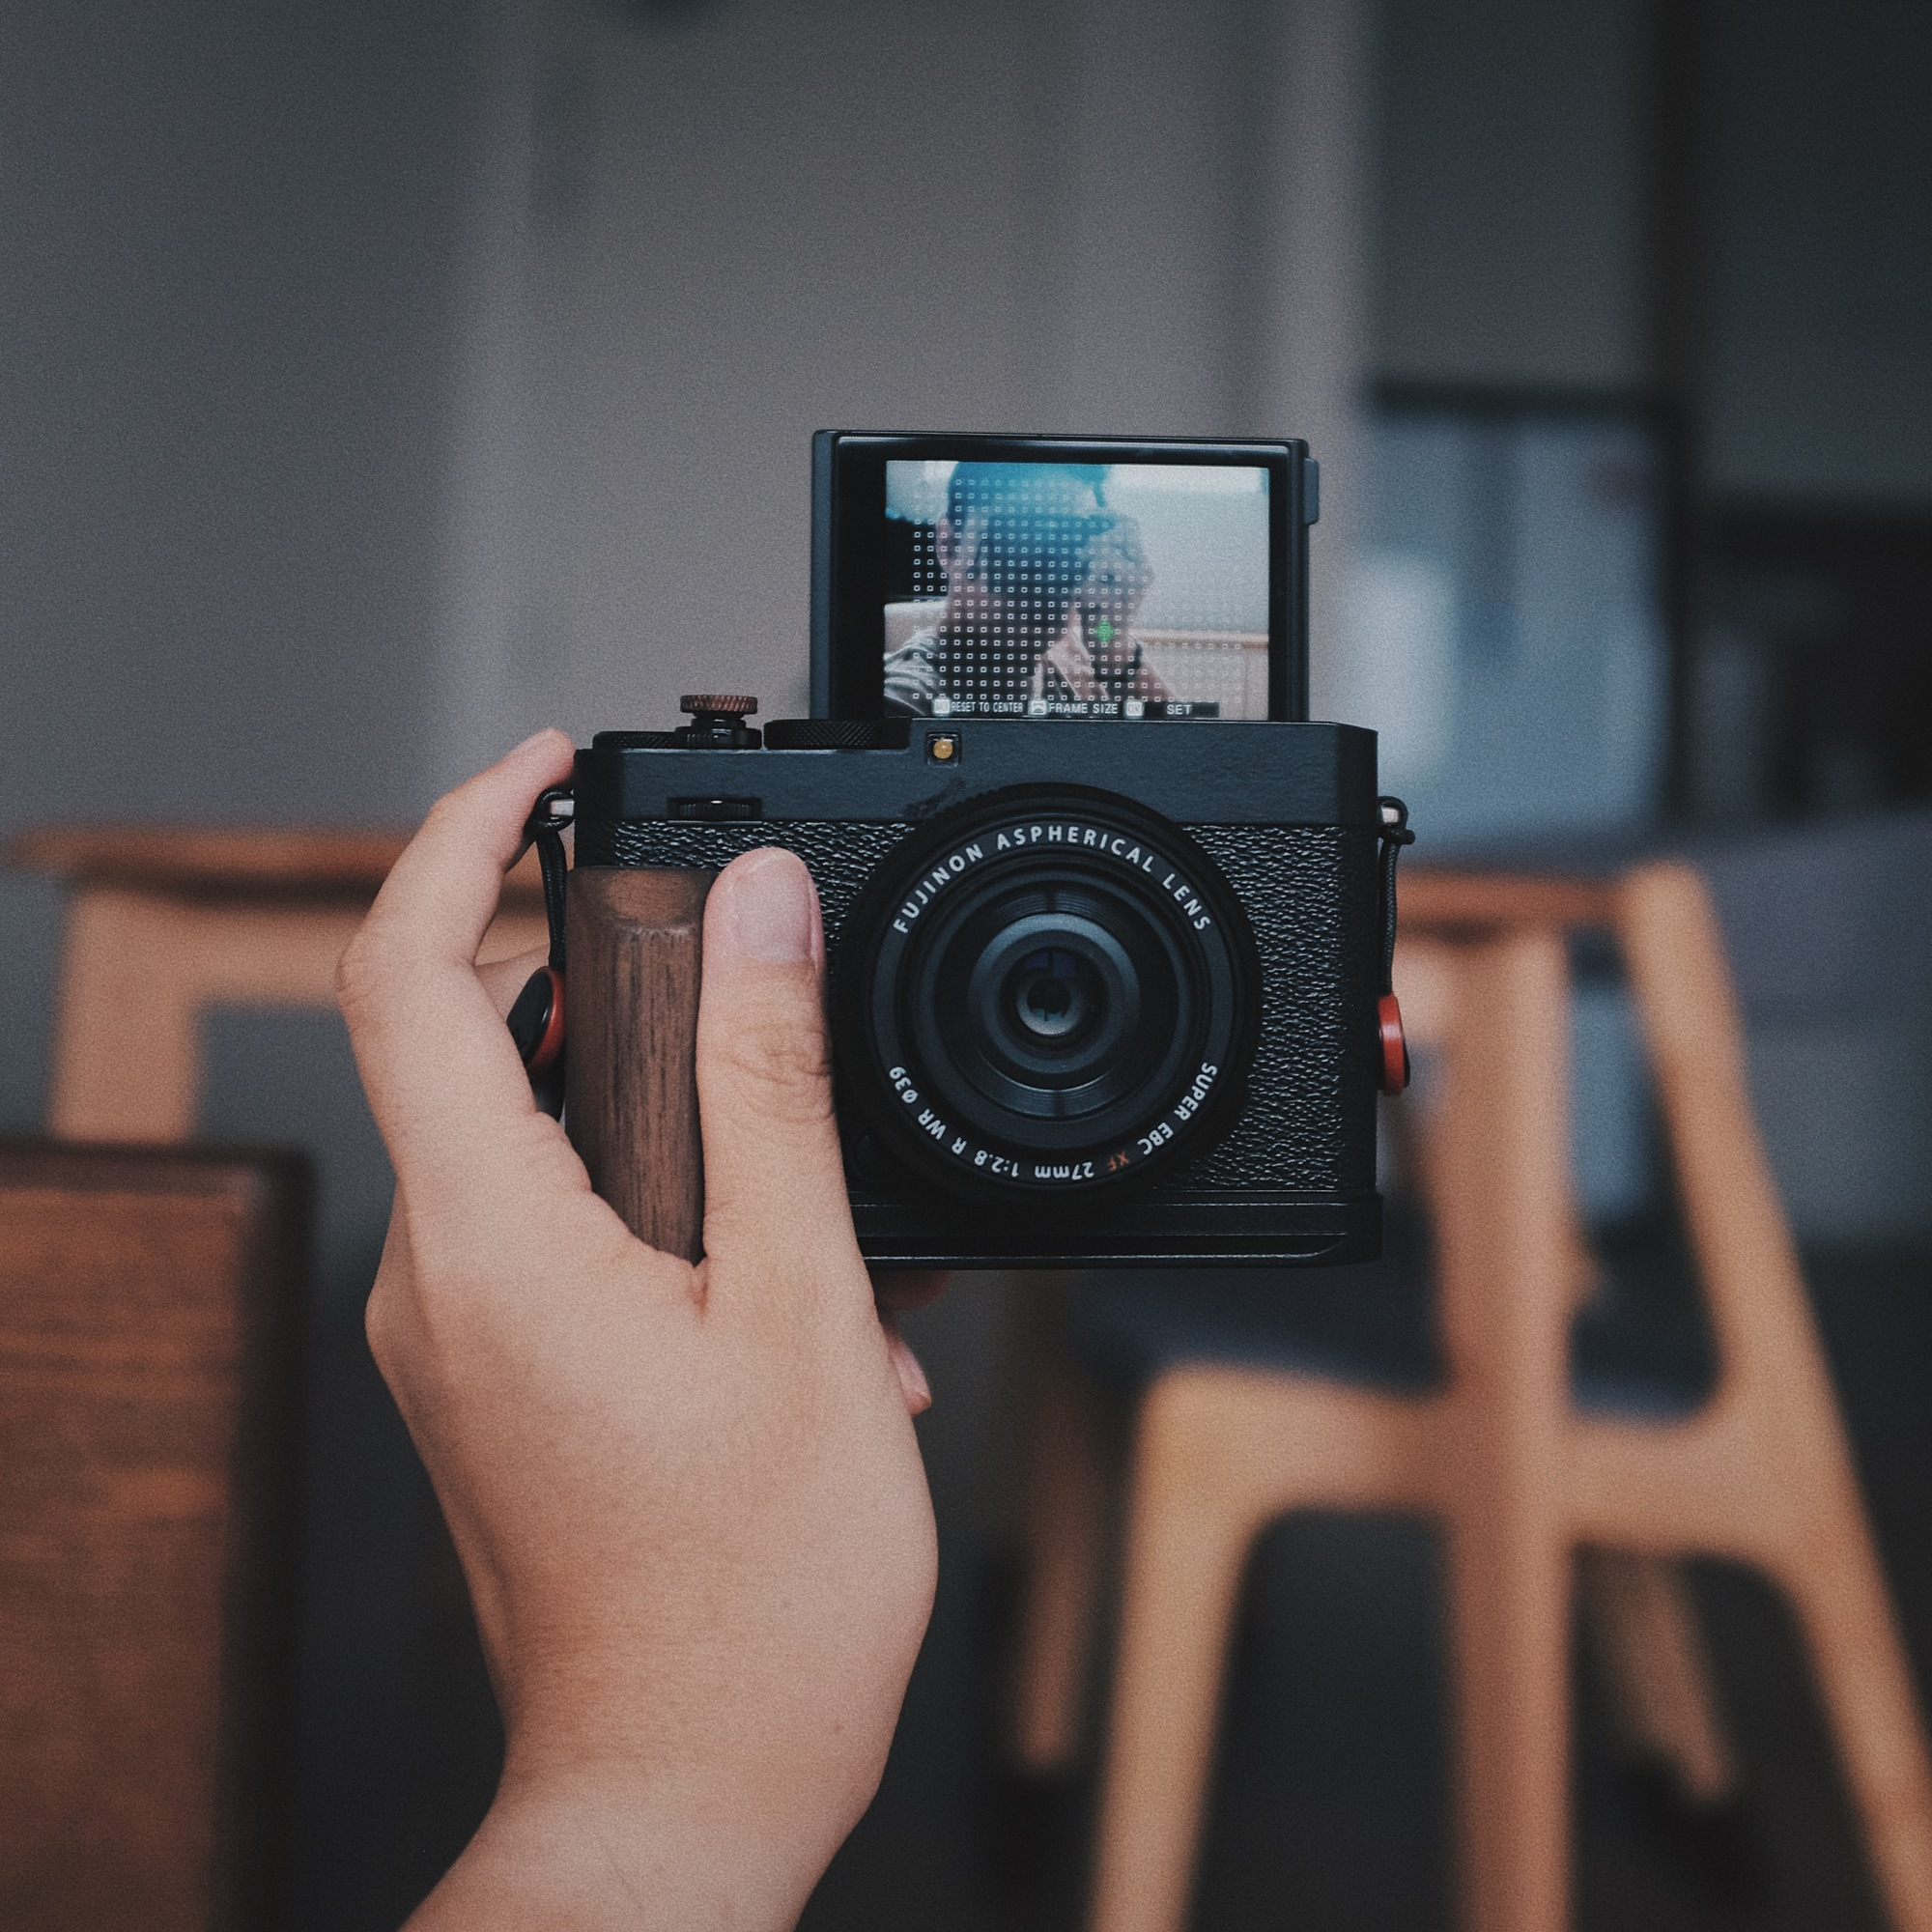
\includegraphics[width=\linewidth]{\envfinaldir/coverpic-prod.jpg}\par
            % \vskip 30pt
            \vfill

            \normalsize\rmfamily\scshape
            \copyright{} The Web Digest Project \hfill\large \envdatestr
        \end{center}
    \end{titlepage}
    % \restoregeometry
}
\newcommand{\simplehref}[1]{%
    \textcolor{blue!80!green}{\href{#1}{#1}}%
}
\renewcommand{\contentsname}{\center\Huge\sffamily\bfseries Contents\par\vskip 20pt}
\newcounter{ipartcounter}
\setcounter{ipartcounter}{0}
\newcommand{\ipart}[1]{
    % \vskip 20pt
    \clearpage
    \stepcounter{ipartcounter}
    \phantomsection
    \addcontentsline{toc}{chapter}{#1}
    % \begin{center}
    %     \Huge
    %     \sffamily\bfseries
    %     #1
    % \end{center}
    % \vskip 20pt plus 7pt
}
\newcounter{ichaptercounter}
\setcounter{ichaptercounter}{0}
\newcommand{\ichapter}[1]{
    % \vskip 20pt
    \clearpage
    \stepcounter{ichaptercounter}
    \phantomsection
    \addcontentsline{toc}{section}{\numberline{\arabic{ichaptercounter}}#1}
    \begin{center}
        \Huge
        \sffamily\bfseries
        #1
    \end{center}
    \vskip 20pt plus 7pt
}
\newcommand{\entrytitlefont}[1]{\subsection*{\raggedright\Large\sffamily\bfseries#1}}
\newcommand{\entryitemGeneric}[2]{
    % argv: title, url
    \parbox{\linewidth}{
        \entrytitlefont{#1}\par\vskip 5pt
        \footnotesize\ttfamily\mdseries
        \simplehref{#2}
    }\vskip 11pt plus 11pt minus 1pt
}
\newcommand{\entryitemGithub}[3]{
    % argv: title, url, desc
    \parbox{\linewidth}{
        \entrytitlefont{#1}\par\vskip 5pt
        \footnotesize\ttfamily\mdseries
        \simplehref{#2}\par\vskip 5pt
        \small\rmfamily\mdseries#3
    }\vskip 11pt plus 11pt minus 1pt
}
\newcommand{\entryitemAp}[3]{
    % argv: title, url, desc
    \parbox{\linewidth}{
        \entrytitlefont{#1}\par\vskip 5pt
        \footnotesize\ttfamily\mdseries
        \simplehref{#2}\par\vskip 5pt
        \small\rmfamily\mdseries#3
    }\vskip 11pt plus 11pt minus 1pt
}
\newcommand{\entryitemHackernews}[3]{
    % argv: title, hnurl, rawurl
    % \parbox{\linewidth}{
    %     \entrytitlefont{#1}\par\vskip 5pt
    %     \footnotesize\ttfamily\mdseries
    %     \simplehref{#3}\par
    %     \textcolor{black!50}{\href{#2}{#2}}
    % }\vskip 11pt plus 11pt minus 1pt
    \begin{minipage}{\linewidth}
            \entrytitlefont{#1}\par\vskip 5pt
            \footnotesize\ttfamily\mdseries
            \simplehref{#3}\par
            \textcolor{black!50}{\href{#2}{#2}}
    \end{minipage}\par\vskip 11pt plus 11pt minus 1pt
}







\begin{document}

\makeheader

\tableofcontents\clearpage




\ipart{Developers}
\ichapter{Hacker News}
\entryitemTwoLinks{Offline.kids – Screen-free activities for kids}{https://news.ycombinator.com/item?id=44789192}{https://offline.kids/}

\entryitemTwoLinks{I asked four former friends why we stopped speaking (2023)}{https://news.ycombinator.com/item?id=44788783}{https://www.vogue.com/article/reconnecting-with-ex-friends}

\entryitemTwoLinks{Show HN: I spent 6 years building a ridiculous wooden pixel display}{https://news.ycombinator.com/item?id=44787902}{https://benholmen.com/blog/kilopixel/}

\entryitemTwoLinks{Tesla withheld data, lied, misdirected police to avoid blame in Autopilot crash}{https://news.ycombinator.com/item?id=44787780}{https://electrek.co/2025/08/04/tesla-withheld-data-lied-misdirected-police-plaintiffs-avoid-blame-autopilot-crash/}

\entryitemTwoLinks{Qwen-Image: Crafting with native text rendering}{https://news.ycombinator.com/item?id=44787631}{https://qwenlm.github.io/blog/qwen-image/}

\entryitemTwoLinks{A deep dive into Rust and C memory interoperability}{https://news.ycombinator.com/item?id=44786962}{https://notashes.me/blog/part-1-memory-management/}

\entryitemTwoLinks{AI promised efficiency. Instead, it's making us work harder}{https://news.ycombinator.com/item?id=44786790}{https://afterburnout.co/p/ai-promised-to-make-us-more-efficient}

\entryitemTwoLinks{Objects should shut up}{https://news.ycombinator.com/item?id=44786367}{https://dustri.org/b/objects-should-shut-the-fuck-up.html}

\entryitemTwoLinks{How we made JSON.stringify more than twice as fast}{https://news.ycombinator.com/item?id=44786005}{https://v8.dev/blog/json-stringify}

\entryitemTwoLinks{PHP: The Toyota Corolla of programming}{https://news.ycombinator.com/item?id=44785759}{https://deprogrammaticaipsum.com/the-toyota-corolla-of-programming/}

\entryitemTwoLinks{Perplexity is using stealth, undeclared crawlers to evade no-crawl directives}{https://news.ycombinator.com/item?id=44785636}{https://blog.cloudflare.com/perplexity-is-using-stealth-undeclared-crawlers-to-evade-website-no-crawl-directives/}

\entryitemTwoLinks{Read your code}{https://news.ycombinator.com/item?id=44785562}{https://etsd.tech/posts/rtfc/}

\entryitemTwoLinks{My Ideal Array Language}{https://news.ycombinator.com/item?id=44785224}{https://www.ashermancinelli.com/csblog/2025-7-20-Ideal-Array-Language.html}

\entryitemTwoLinks{Century-old stone ``tsunami stones'' dot Japan's coastline (2015)}{https://news.ycombinator.com/item?id=44785107}{https://www.smithsonianmag.com/smart-news/century-old-warnings-against-tsunamis-dot-japans-coastline-180956448/}

\entryitemTwoLinks{DrawAFish.com Postmortem}{https://news.ycombinator.com/item?id=44784743}{https://aldenhallak.com/blog/posts/draw-a-fish-postmortem.html}

\entryitemTwoLinks{Palantir is extending its reach even further into government}{https://news.ycombinator.com/item?id=44784498}{https://www.wired.com/story/palantir-government-contracting-push/}

\entryitemTwoLinks{KDE Plasma prepares crackdown on focus-stealing window behavior under Wayland}{https://news.ycombinator.com/item?id=44784312}{https://www.neowin.net/news/kde-plasma-prepares-crackdown-on-focus-stealing-window-behavior-under-wayland/}

\entryitemTwoLinks{GHz spiking neuromorphic photonic chip with in-situ training}{https://news.ycombinator.com/item?id=44784297}{https://arxiv.org/abs/2506.14272}

\entryitemTwoLinks{Mastercard deflects blame for NSFW games being taken down}{https://news.ycombinator.com/item?id=44783566}{https://www.pcgamer.com/games/mastercard-deflects-blame-for-nsfw-games-being-taken-down-but-valve-says-payment-processors-specifically-cited-a-mastercard-rule-about-damaging-the-brand/}

\entryitemTwoLinks{HTMX is hard, so let's get it right}{https://news.ycombinator.com/item?id=44783266}{https://github.com/BookOfCooks/blog/blob/master/htmx-is-hard-so-lets-get-it-right.md}


\ipart{Developers~~~~(zh-Hans)}
\ichapter{Solidot}
\entryitemGeneric{\hskip 0pt{}ISS 俄罗斯舱仍在漏气}{https://www.solidot.org/story?sid=81956}

\entryitemGeneric{\hskip 0pt{}Steam 用户中 Linux 比例接近 3\%}{https://www.solidot.org/story?sid=81955}

\entryitemGeneric{\hskip 0pt{}印度将惩罚论文撤稿太多的大学}{https://www.solidot.org/story?sid=81954}

\entryitemGeneric{\hskip 0pt{}比利时限制访问互联网档案馆的在线图书馆 }{https://www.solidot.org/story?sid=81953}

\entryitemGeneric{\hskip 0pt{}Google 改变关闭 goo.gl 短链接的计划}{https://www.solidot.org/story?sid=81952}

\entryitemGeneric{\hskip 0pt{}17 岁的 Hannah Cairo 解决了有 40 年历史的数学猜想}{https://www.solidot.org/story?sid=81951}

\entryitemGeneric{\hskip 0pt{}美国政客的年龄比其他国家都年长}{https://www.solidot.org/story?sid=81950}\ichapter{V2EX}
\entryitemGeneric{\hskip 0pt{}[Apple] 把照片图库迁移到外置硬盘后,照片.app 不能勾选 iCloud 照片。}{https://www.v2ex.com/t/1149942}

\entryitemGeneric{\hskip 0pt{}[问与答] 初一的孩子一脸青春痘 有什么办法缓解吗}{https://www.v2ex.com/t/1149941}

\entryitemGeneric{\hskip 0pt{}[问与答] 新版 Mac 微信,怎么关闭长按 cmd-Q 退出?}{https://www.v2ex.com/t/1149940}

\entryitemGeneric{\hskip 0pt{}[职场话题] 今天终面线下见总监理,还没有发 offer,但…}{https://www.v2ex.com/t/1149938}

\entryitemGeneric{\hskip 0pt{}[macOS] 输入英文单词 重复输入 原因 排查求助`}{https://www.v2ex.com/t/1149937}

\entryitemGeneric{\hskip 0pt{}[Node.js] [北京/南京/hybrid] AI 出海 APP 找长期后端兼职 supabase+graghQL 600-1000 元/天}{https://www.v2ex.com/t/1149934}

\entryitemGeneric{\hskip 0pt{}[Solana] 虚拟小白提问 2,\$V2EX 是用 SOL 做 gas 费, SOL 一直涨的话,那么 gas 费就会涨,那 Solana 交易费用低的优势不就不复存在了吗?}{https://www.v2ex.com/t/1149933}

\entryitemGeneric{\hskip 0pt{}[程序员] udemy 上面的课程值得学吗?}{https://www.v2ex.com/t/1149931}

\entryitemGeneric{\hskip 0pt{}[React] 来个专业写 移动 web 前端的, React}{https://www.v2ex.com/t/1149929}

\entryitemGeneric{\hskip 0pt{}[分享创造] [自荐] 做了一个 json diff 工具站,但是能支持 key 顺序不一致的情况进行 diff}{https://www.v2ex.com/t/1149928}

\entryitemGeneric{\hskip 0pt{}[酷工作] [兼职] 抖音在线云客服}{https://www.v2ex.com/t/1149926}

\entryitemGeneric{\hskip 0pt{}[Go 编程语言] 谁用过 livekit 通信框架}{https://www.v2ex.com/t/1149924}

\entryitemGeneric{\hskip 0pt{}[职场话题] base 低进大厂还会卡涨幅吗}{https://www.v2ex.com/t/1149922}

\entryitemGeneric{\hskip 0pt{}[云修电脑] 主力 PC 独立显卡丢了}{https://www.v2ex.com/t/1149920}

\entryitemGeneric{\hskip 0pt{}[问与答] 如何对用户上传的图片进行合规性检查?}{https://www.v2ex.com/t/1149919}

\entryitemGeneric{\hskip 0pt{}[Solana] 不懂就问,在交易所交易 V2EX 和在钱包交易 V2EX 有什么区别吗?}{https://www.v2ex.com/t/1149918}

\entryitemGeneric{\hskip 0pt{}[Solana] 请教一个\$V2EX 的技术细节}{https://www.v2ex.com/t/1149917}

\entryitemGeneric{\hskip 0pt{}[程序员] indextts 的语音 确实挺不错,部署多卡应该不是这样吧}{https://www.v2ex.com/t/1149916}

\entryitemGeneric{\hskip 0pt{}[问与答] 感觉现在 115 的磁链离线比迅雷有差距了}{https://www.v2ex.com/t/1149915}

\entryitemGeneric{\hskip 0pt{}[奇思妙想] 有没有能记录看书进度的 APP}{https://www.v2ex.com/t/1149914}

\entryitemGeneric{\hskip 0pt{}[问与答] 有在用 vnstat 工具统计流量的吗?}{https://www.v2ex.com/t/1149913}

\entryitemGeneric{\hskip 0pt{}[Solana] 教程:入场持有社区代币\$V2EX}{https://www.v2ex.com/t/1149911}

\entryitemGeneric{\hskip 0pt{}[阅读] 阅读书籍,是不是改变大脑最好的方法?}{https://www.v2ex.com/t/1149910}

\entryitemGeneric{\hskip 0pt{}[问与答] 求支付宝菜鸟小程序域名规则}{https://www.v2ex.com/t/1149909}

\entryitemGeneric{\hskip 0pt{}[Solana] 插个眼,支持 200U}{https://www.v2ex.com/t/1149908}

\entryitemGeneric{\hskip 0pt{}[杭州] 如果现在买房,作为程序员,应该买在哪里呢?良渚还是崇贤呢?}{https://www.v2ex.com/t/1149907}

\entryitemGeneric{\hskip 0pt{}[程序员] 请问 saas 平台是怎么防止攻击和刷流量的?}{https://www.v2ex.com/t/1149906}

\entryitemGeneric{\hskip 0pt{}[分享发现] jms 堡垒机企业版疑似被破解了}{https://www.v2ex.com/t/1149905}

\entryitemGeneric{\hskip 0pt{}[职场话题] 都是 25k,这两家公司如何选择?}{https://www.v2ex.com/t/1149904}

\entryitemGeneric{\hskip 0pt{}[求职] 💼 全栈开发 · 8 年经验 · 接单中}{https://www.v2ex.com/t/1149903}

\entryitemGeneric{\hskip 0pt{}[问与答] 阿里云购买的域名可以转到 cf 上吗}{https://www.v2ex.com/t/1149902}

\entryitemGeneric{\hskip 0pt{}[Solana] 充了 100R 支持了一下,短短 2 小时,赚了\$2}{https://www.v2ex.com/t/1149900}

\entryitemGeneric{\hskip 0pt{}[分享创造] 摸鱼福利网站接入 GPT 绘画}{https://www.v2ex.com/t/1149899}

\entryitemGeneric{\hskip 0pt{}[求职] 8 年工作经验,目前国企前端负责人,求个网易内推,或其它公司内推,感谢!}{https://www.v2ex.com/t/1149898}

\entryitemGeneric{\hskip 0pt{}[汽车] 理想车主真的大部分素质堪忧吗}{https://www.v2ex.com/t/1149897}

\entryitemGeneric{\hskip 0pt{}[分享发现] 钱越来越难挣了,股票收益都不如税高....}{https://www.v2ex.com/t/1149896}

\entryitemGeneric{\hskip 0pt{}[旅行] 想花半个月从成都自驾去新疆,求建议}{https://www.v2ex.com/t/1149895}

\entryitemGeneric{\hskip 0pt{}[VPS] vps 防火墙关闭了 ping,各位在保护自己服务器上还有哪些高招求指点}{https://www.v2ex.com/t/1149894}

\entryitemGeneric{\hskip 0pt{}[天黑以后] 20250804 午夜俱乐部}{https://www.v2ex.com/t/1149889}

\entryitemGeneric{\hskip 0pt{}[ WATCH] 2 月份买的 Apple Watch S10 掉漆了💔}{https://www.v2ex.com/t/1149888}

\entryitemGeneric{\hskip 0pt{}[新手求助] 连续签到一年,问问这个铜币有啥用?}{https://www.v2ex.com/t/1149886}

\entryitemGeneric{\hskip 0pt{}[上海] [转租]嘉定新城白银路电梯房 2700 2 室 1 厅 70 平}{https://www.v2ex.com/t/1149885}

\entryitemGeneric{\hskip 0pt{}[问与答] 帮忙,这种忙你怎么帮}{https://www.v2ex.com/t/1149883}

\entryitemGeneric{\hskip 0pt{}[DNS] 请教下这种域名是什么作用,是否是恶意域名}{https://www.v2ex.com/t/1149882}

\entryitemGeneric{\hskip 0pt{}[分享创造] 写了个在 YouTube 上自动同步显示 B 站弹幕的 Chrome 插件}{https://www.v2ex.com/t/1149881}

\entryitemGeneric{\hskip 0pt{}[程序员] 做了个可以将 soundcloud.com 音乐下载为 mp3 的小工具,欢迎试用}{https://www.v2ex.com/t/1149879}

\entryitemGeneric{\hskip 0pt{}[汽车] 2025 年 8 月, 8w 预算,想搞一台纯油车,最佳选择是?}{https://www.v2ex.com/t/1149878}

\entryitemGeneric{\hskip 0pt{}[Apple] 苹果妙控板 2, 3 代有啥区别?白色和黑色呢?}{https://www.v2ex.com/t/1149877}

\entryitemGeneric{\hskip 0pt{}[NGINX] 问问大家 nginx 日志流量分析用什么方案?}{https://www.v2ex.com/t/1149876}

\entryitemGeneric{\hskip 0pt{}[投资] 境外买卖股票也要缴税了}{https://www.v2ex.com/t/1149875}


\ipart{Generic News}







\clearpage
\leavevmode\vfill
\footnotesize

Copyright \copyright{} 2023-2025 Neruthes and other contributors.

This document is published with CC BY-NC-ND 4.0 license.

The entries listed in this newsletter may be copyrighted by their respective creators.

This newsletter is generated by the Web Digest project.

The newsletters are also delivered via Telegram channel \CJKunderline{\href{https://t.me/webdigestchannel}{https://t.me/webdigestchannel}}.\\
RSS feed is available at \CJKunderline{\href{https://webdigest.pages.dev/rss.xml}{https://webdigest.pages.dev/rss.xml}}.

This newsletter is available in PDF at
\CJKunderline{\href{https://webdigest.pages.dev/}{https://webdigest.pages.dev/}}.

The source code being used to generate this newsletter is available at\\
\CJKunderline{\href{https://github.com/neruthes/webdigest}{https://github.com/neruthes/webdigest}}.

This newsletter is also available in
\CJKunderline{\href{http://webdigest.pages.dev/readhtml/\envyear/WebDigest-20250805.html}{HTML}} and
\CJKunderline{\href{https://github.com/neruthes/webdigest/blob/master/markdown/\envyear/WebDigest-20250805.md}{Markdown}}.


\coverpic{https://unsplash.com/photos/colorful-houses-stand-beneath-power-lines-al3lRa-emTc}{Linus Belanger}


\end{document}
